\documentclass{beamer}
\usepackage[utf8]{inputenc}

\usetheme{Madrid}
\usecolortheme{default}
\usepackage{amsmath,amssymb,amsfonts,amsthm}
\usepackage{txfonts}
\usepackage{tkz-euclide}
\usepackage{listings}
\usepackage{adjustbox}
\usepackage{array}
\usepackage{tabularx}
\usepackage{gvv}
\usepackage{lmodern}
\usepackage{circuitikz}
\usepackage{tikz}
\usepackage{graphicx}

\setbeamertemplate{page number in head/foot}[totalframenumber]

\usepackage{tcolorbox}
\tcbuselibrary{minted,breakable,xparse,skins}



\definecolor{bg}{gray}{0.95}
\DeclareTCBListing{mintedbox}{O{}m!O{}}{%
  breakable=true,
  listing engine=minted,
  listing only,
  minted language=#2,
  minted style=default,
  minted options={%
    linenos,
    gobble=0,
    breaklines=true,
    breakafter=,,
    fontsize=\small,
    numbersep=8pt,
    #1},
  boxsep=0pt,
  left skip=0pt,
  right skip=0pt,
  left=25pt,
  right=0pt,
  top=3pt,
  bottom=3pt,
  arc=5pt,
  leftrule=0pt,
  rightrule=0pt,
  bottomrule=2pt,

  colback=bg,
  colframe=orange!70,
  enhanced,
  overlay={%
    \begin{tcbclipinterior}
    \fill[orange!20!white] (frame.south west) rectangle ([xshift=20pt]frame.north west);
    \end{tcbclipinterior}},
  #3,
}
\lstset{
    language=C,
    basicstyle=\ttfamily\small,
    keywordstyle=\color{blue},
    stringstyle=\color{orange},
    commentstyle=\color{green!60!black},
    numbers=left,
    numberstyle=\tiny\color{gray},
    breaklines=true,
    showstringspaces=false,
}
%------------------------------------------------------------
%This block of code defines the information to appear in the
%Title page
\title %optional
{1.4.28}
\date{August  2025}
%\subtitle{A short story}

\author % (optional)
{BEERAM MADHURI - EE25BTECH11012}



\begin{document}


\frame{\titlepage}
\begin{frame}{Question}
 Find the position vector of a point $\mathbf{R}$ which divides the line joining two points $\mathbf{P}$ and $\mathbf{Q}$ whose position vectors are $(2\mathbf{a} + \mathbf{b})$ and $(\mathbf{a} - 3\mathbf{b})$ externally in the ratio $1 : 2$. Also, show that $\mathbf{P}$ is the mid point of the line segment $RQ$.
 
 

\end{frame}
 
\begin{frame}{given data}
 
\text \textbf{R} divides \textbf{p} and \textbf{Q} in 1:2 ratio.
\[
\begin{array}{|c|c|c|c|}
\hline
\textbf{variable} & \textbf{Position Vector}\\
\hline
\textbf{P} & 2a+b\\
\textbf{Q} & a-3b\\
\hline
\end{array}
\]

   
\end{frame}

\begin{frame}{Formula}
Section Formula for a vector 
  \textbf{R} which divides \textbf{P} and \textbf{Q} in k:1 ratio externally is given by 

\begin{align*}
 \textbf{R} &= \frac{k(\textbf{P}) - 1(\textbf{Q})}{k - 1}
 \end{align*}
 \end{frame}
 

\begin{frame}{solution}
    \frametitle{finding Position vector of \textbf{R}}
\begin{align}
    \textbf{R} &= \frac{2(\textbf{P}) - 1(\textbf{Q})}{2 - 1} \\
&= \frac{2(2a+b) - (a-3b)}{1} \\
&= 3a + 5b\\
\end{align}
Hence Position vector of \textbf{R} is 3a + 5b
\end{frame}
\begin{frame}{solution}
    \frametitle{Proving \textbf{P} is midpoint of \textbf{QR}
    \begin{align*}
\textbf{P} &= \frac{k(\textbf{R}) + 1(\textbf{Q})}{k+1} \\
2a+b &= \frac{k(3a+5b) + a-3b}{k+1} \\
(2a+b)(k+1) &= (3k+1)a + (5k-3)b
\end{align*}
\text{Comparing coefficients of } a:
\begin{align*}
2k+2 &= 3k+1 \\
k &= 1
\end{align*}

\text Hence \textbf{P} divides $\overline{RQ}$ in 1:1 ratio, P is midpoint of $\overline{RQ}$.

\end{frame}


\begin{frame}[fragile]
    \frametitle{Python Code}
    \begin{lstlisting}
 import matplotlib.pyplot as plt
import numpy as np

#  Define Base Vectors
# We assign arbitrary coordinates to vectors 'a' and 'b' for visualization.
# To see a different layout, you can change these values.
a = np.array([1, 1])
b = np.array([-1, 2])

\end{lstlisting}
\end{frame}

\begin{frame}[fragile]
    \frametitle{Python Code}

    \begin{lstlisting}
#  Define Position Vectors for P and Q
# As given in the problem statement.
P = 2*a + b
Q = a - 3*b

    \end{lstlisting}
\end{frame}

\begin{frame}[fragile]
    \frametitle{Python Code}

    \begin{lstlisting}
 # Calculate Position Vector for R ---
# Using the external division formula result we found: R = 3a + 5b
R = 3*a + 5*b
    \end{lstlisting}
\end{frame}

\begin{frame}[fragile]
    \frametitle{Python Code}

    \begin{lstlisting}
# Verify P is the midpoint of RQ ---
# This calculation should result in the same coordinates as P.
midpoint_RQ = (R + Q) / 2
print(f"Coordinates of P: {P}")
print(f"Calculated midpoint of RQ: {midpoint_RQ}")
print(f"Is P the midpoint of RQ? {np.allclose(P, midpoint_RQ)}")

\end{lstlisting}
\end{frame}

 
\begin{frame}[fragile]
    \frametitle{Python Code}

    \begin{lstlisting}
# --- Create the Plot ---
fig, ax = plt.subplots(figsize=(10, 8))

# Plot the line segment RQ
ax.plot([R[0], Q[0]], [R[1], Q[1]], 'k--', alpha=0.6, label='Line Segment RQ')

# Plot the points O, P, Q, R
ax.scatter(0, 0, c='black', s=100, zorder=5, label='Origin (O)')
ax.scatter(P[0], P[1], c='red', s=100, zorder=5, label=f'P = {P}')
ax.scatter(Q[0], Q[1], c='green', s=100, zorder=5, label=f'Q = {Q}')
ax.scatter(R[0], R[1], c='blue', s=100, zorder=5, label=f'R = {R}')


# Plot position vectors from the origin
ax.quiver(0, 0, P[0], P[1], angles='xy', scale_units='xy', scale=1, color='red', alpha=0.7)
ax.quiver(0, 0, Q[0], Q[1], angles='xy', scale_units='xy', scale=1, color='green', alpha=0.7)
ax.quiver(0, 0, R[0], R[1], angles='xy', scale_units='xy', scale=1, color='blue', alpha=0.7)
\end{lstlisting}
\end{frame}
\begin{frame}[fragile]
    \frametitle{Python Code}

    \begin{lstlisting}
# Add Labels and Formatting 
# Add text labels for each point
ax.text(0, 0.5, 'O', fontsize=14)
ax.text(P[0] + 0.3, P[1], 'P', fontsize=14)
ax.text(Q[0] + 0.3, Q[1], 'Q', fontsize=14)
ax.text(R[0] + 0.3, R[1], 'R', fontsize=14)


# Set plot aesthetics
ax.set_title('Vector Visualization', fontsize=16)
ax.set_xlabel('X-axis', fontsize=12)
ax.set_ylabel('Y-axis', fontsize=12)
ax.axhline(0, color='grey', linewidth=0.5)
ax.axvline(0, color='grey', linewidth=0.5)
ax.grid(True, which='both', linestyle='--', linewidth=0.5)
ax.set_aspect('equal', adjustable='box')
ax.legend()

plt.show()
\end{lstlisting}
\end{frame}




\begin{frame}[fragile]
\frametitle{C Code}
\begin{lstlisting}
  
#include <stdio.h>

// A structure to represent a vector with coefficients for a and b
typedef struct {
    int coeff_a;
    int coeff_b;
} Vector;

int main() {
    // P = 2a + 1b
    Vector P = {2, 1};
    // Q = 1a - 3b
    Vector Q = {1, -3};
    // Ratio m:n = 1:2
    int m = 1;
    int n = 2;

    // Applying the external division formula: R = (m*Q - n*P) / (m - n)
    
    // Numerator: (1 * Q) - (2 * P)
    int num_a = (m * Q.coeff_a) - (n * P.coeff_a); // (1*1) - (2*2) = -3
    int num_b = (m * Q.coeff_b) - (n * P.coeff_b); // (1*-3) - (2*1) = -5

    // Denominator: m - n
    int den = m - n; // 1 - 2 = -1
    Vector R;
    R.coeff_a = num_a / den; // -3 / -1 = 3
    R.coeff_b = num_b / den; // -5 / -1 = 5

    printf("The position vector of point R is (%d)a + (%d)b\n", R.coeff_a, R.coeff_b);
return 0;
}

\end{lstlisting}

\end{frame}


\begin{frame}[fragile]
\frametitle{Python and C Code}

\begin{lstlisting}
import subprocess

# 1. Compile the C program
subprocess.run(["gcc", "vector_division.c", "-o", "vector_division"])

# 2. Run the compiled C program
result = subprocess.run(["./vector_division"], capture_output=True, text=True)

# 3. Print the output from the C program
print(result.stdout)
\end{lstlisting}

\end{frame}

 


\begin{figure}
    \centering
    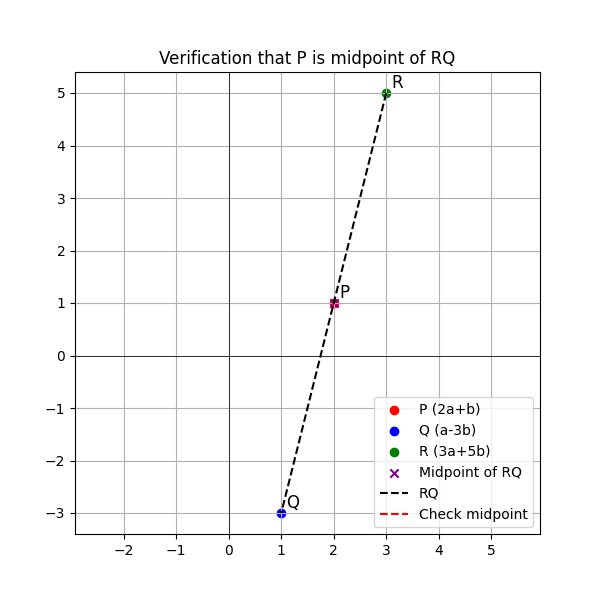
\includegraphics[width=0.75\columnwidth]{Fig.png}
    \caption{Plot}
    \label{fig:placeholder}
\end{figure}


\end{document}